% TODO change this uglyness
\chapter{The Serial Replication in \ak\ }

In this chapter we explain the machinery behind the serial replication in \ak\ and the role of synchronisers in it.
%TODO
%First of all, the semantics of AstraKahn on the TPL is described in terms of structures put in place for the coordinator, i.e. a controlling agent, or indeed a group of agents, responsible for progress and communication of the KPN vertices.
%
%The rest of the chapter is organised as follows. In sections \ref{ffp} and \ref{rfp} we explain why both cases are relevant to synchroniser analysis and give formal definitions. In section \ref{ffp_discussion} we discuss the original approach to the output of the infinite chain of replicas and in section \ref{approach} we propose another one. In section \ref{fp_detect} we provide detection algoritms for both cases.


    \section{Motivation}
The serial replication combinator creates conceptually infinite number of copies of its operand network, and connects them in a chain. Replication is demand-driven, hence replicas are created dynamically in runtime. A fresh replica is \emph{inactive}\footnote{More generally, we call a replica inactive when all of its synchronisers are in their start states, none of its channels has messages in them and no box is running}, hence it does not necessarily require significant resouces since \ak\ boxes are stateless and synchronisers require no resouces in their start state\footnote{When a synchroniser transitions back to the start state, it flushes its store variables}. Indeed the cost of replication is only felt when the replicas are active, which is the case when the first message is received until all messages have left the replica and all its synchronisers have returned to their start states.

%loop construct with pipeline parallelism

    \section{\ak\ Approach to the Serial Replication}

In S-Net, the output from the replication pipeline is based on the record subtyping in the type system. The replication combinators in S-Net require the programmer to specify a termination pattern, so that each record that is a subtype of this pattern leaves the replication pipeline throught the output stream. In \ak\, a message leaves the replication pipeline exclusively via a special complement channel that is wired to the rest of the \ak\ network. The programmer has to make sure that the messages to be sent on are detected within the operand network and sent to this channel. 
Thus, the serial replication in \ak\ enforces a topological property of the operand network that is formally defined as follows. Consider the serial replication $N^{*}$ of an operand network $N$ with the input and output channel sets $\mathcal{I}$ and $\mathcal{O}$ respectively. Consequently, the set of matched inputs and outputs is $\mathcal{M}(\mathcal{I}, \: \mathcal{O}) = \mathcal{I} \cap \mathcal{O}$. In order for the serial replication $N^{*}$ to be able to produce output to the channel $x \in \mathcal{M}(\mathcal{I}, \: \mathcal{O})$, at least one box or a synchroniser in $N$ must have the output port wired to the complement channel $x'$. The \ak\ compiler recognizes the use of complement channels and checks whether the operand network topology has this property. If it does not, the compiler reports an error and aborts the compilation.

The \ak\ runtime is committed to support the dynamic rewiring for complement channels. The serial replication implementation depends on the \ak\ runtime implementation, particularly the primitives the runtime system provides for the network construction. We briefly describe two approaches to the serial replication implementation with respect to the available primitives.


The first approach relies on a port wiring primitive $P$ that transmits messages immediately from one port to another without storing them. The operand network $A$ in Fig. \ref{fig:ffp_new} has a single input port $x$ and two output ports. The output port $x$ is intended for the messages that proceed to the the next replica of $A$ in the chain, and the output port $x'$ is a complement port for the messages that are supposed to leave the replication pipeline. The serial replication network $A^{*}$ has a single input and a single output port both named $x$. During the compilation, the operand network $A$ is encapsulated into the special network $N$ it as shown in Fig. \ref{fig:ffp_new}. The network $N$ inherits all the ports from $A$ and adds a corresponding input port $x'$. The input and output ports $x'$ of $N$ are connected with the wiring primitive $P$. The output and the input ports $x'$ of the consequent replicas of $N$ are connected with the wiring primitive $P$ as well.
\begin{figure}[h!]
\centering
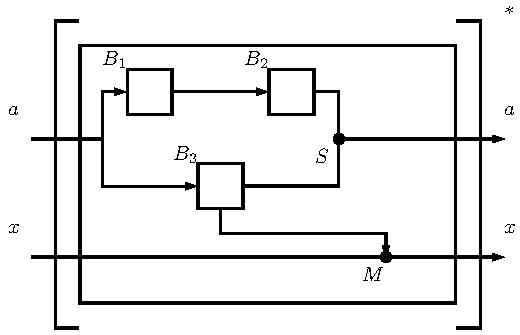
\includegraphics[scale=0.8]{figs/chapter_04_ffp_new.pdf}
\caption{The operand network $A$ (top) and a possible implementation of its serial replication $A^{*}$ (bottom)}
\label{fig:ffp_new}
\end{figure}
A message that $A$ sends to the output port $x'$ cascades through all the active replicas. Once it has reached an inactive replica, the output channel $x$ of $A^{*}$ is dynamically wired to the output port $x'$ of the last active replica of $N$. When the replica becomes active, the port $x'$ is rewired with the input port of this replica using $P$.

The second approach to the serial replication implementation relies on a merger with variable number of inputs. When a replica of $A$ sends a message to the output port $x'$, a new input channel is created for the merger $M$ and wired to the output port $x'$ of the replica as shown in Fig. \ref{fig:ffp_new_1}. The merger's output port is wired to the output channel $x$ of $A^{*}$.
\begin{figure}[h]
\centering
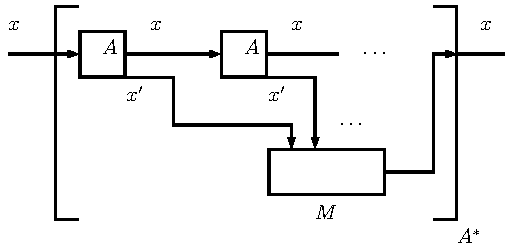
\includegraphics[scale=0.8]{figs/chapter_04_ffp_new_1.pdf}
\caption{Another possible implementation of the serial replication $A^{*}$}
\label{fig:ffp_new_1}
\end{figure}

%The serial replication implements a loop with variable tripcount

    \section{An example}
% TODO: I don't like the reason. Why was the reverse fixed point introduced?
% reverse fixed point is the basic optimisation that preserves growth of the replicas chain.
In order to supress the growth of the replicas chain


As the chain of replicas evolves, it may be the case that some replicas in the head of the chain are active yet they just transmit messages without a change. \ak\ is commited to detect such replicas and optimise the connection so that the data are sent directly to a replica that is ready to process it. 



%\ak\ provides a termination mechanism that does not require to explicitly specify termination rules in the \ak\ application code. This mechanism is inspired by the concept of a fixed point.
%
%In mathematics, a fixed point of a function is an element of the function's domain that is mapped to itself by the function. Mapping this definition to messages and components we obtain the fixpoint definition of an \ak\ net: a message that leaves a net inactive after it was processed is called a fixpoint of the given \ak\ net. (NOT TRUE, FIX)
%
%TODO!! Explain that synchroniser analysis is relevant to fix-point resolution
%In order to utilize the fixed point the \ak\ compiler must be able to detect it. Due to separation of concerns \ak\ does not have to analyse the box code\footnote{except for CAL passport generation}, therefore the fixed point must be defined in synchronisers or the network topology of a net. It means that the net graph must have at least one path that goes exclusively via synchronisers (TODO fix) or straight through the net without traversing any box.
%
%\ak\ defines two types of a fixed point: a forward fixed point and a reverse fixed point. The intention of a forward fixed point is to cut infinite tail of inactive replicas chain. The reverse fixed point is an optimisation of an input connection that has to cascade through the chain to a replica that is ready to accept the data. Its intention is to bypass the replicas that transmit messages without change (TODO not good). Later we will see that a replica does not have to be inactive in order to that.
%
%With the reference to fixed point utilisation we will call the \ak\ replication operator the fixed point series (FPS).





    \section{Reverse Fixed Point Series\label{rfp}}
%channels are ordered, need to insert synchronisers
In this section we provide the approach to the reverse fixed point.

Consider a vertex $v$ that has an input and an output channel, both named $x$.

\begin{definition} The vertex $v$ is said to have a reverse fixed point in $x$ if and only if the following statements hold:

\begin{enumerate}
\item A unique non-branching path from the input to the output channel $x$ exists that does not traverse any boxes.

\item Every synchroniser $S_i$ on the path has a subset of states, which we denote as $s_i$, such that in each of these states every message on the path is immediately transferred without being changed or even stored, causing the synchroniser to remain in the same state\footnote{It should also be borne in mind that the values of any state variables form a part of the synchroniser state}. In a state from $s_i$ the synchroniser $S_i$ may still be sensitive to other input channels, as long as this does not, under any circumstances, cause a transition to a state outside $s_i$.
\end{enumerate}
\end{definition}

The vertex $v$ is said to be in a reverse fixed point state on channel $x$ when each $S_i$ is in a state that belongs to its $s_i$.

%%%%%%%%%
%%  Motivation for the reverse fixpoint
%%%%%%%%%
The reverse fix-point is defined to unify backslash \ combinatior and the star in terms of their functionality, which was never done in S-Net(TODO which patterns??). The intention is that they only differ in the pressure propagation strategy. The backslash creates no pressure (TODO why??) in its looped channel, and the start mantains and propagates the pressure in channels between instanses.

% probably a picture
%
% backslash (* is the synchroniser)
%      _________
%    \|/ _____  |
% ____*_|     |_|
%       |_____|
%
%
% Star with the reverse fix point
%        __________________
%      _|___________       |
%    _|______       |      |
%   |    __ \|/ __ \|/ __ \|/ __
% --*---|__|-*-|__|-*-|__|-*-|__|-- ...
%

The reverse fix point is more the way to write code. It is the way to program a loop dependency, when the result of the iteration depends not only on the result of the previous iteration but on the new incoming data. The difference with backslash is in the pressure propagation.

If you want the feature, you must define a closed set of translating states in every synchroniser on the fp path.


\subsubsection{Rewiring of the Reverse FPS}
The reverse fixed point optimises an input connection that has to cascade through the chain to a replica that is ready to accept the data. Any input channel $x$ wired to an active replica $A_i$ that transitions to a reverse fixed point state on that channel is disconnected from $A_i$ and dynamically rewired to the input channel $x$ of the next replica on the chain $A'_{i+1}$.

%pic


    \subsection{Discussion}
Order of messages in the reverse fixed point may be changed, because a message may put the replica into the reverse fixed-point state and go for processing into this replica. In this case the messages that came to the replica that is in the reverse fixed-point state may overcome the message processed in the replica. This changes the order of messages. If the progrmmer wants to preserve the order, he must mind it. It may be fixed by creating a separate channel for RFP messages and putting a synchroniser that blockes the RFP channel while there's no message from the output channel (this is for operand network with one input channel, with two it can be more dificult if there're races between the channels that wire replicas).

The replication combinator is just a wiring pattern that does not have to guarantee race-safety. For example, if the operand network is not race-safe, the star is not race-safe as well.


    \subsection{Forward Fixed Point Detection\label{ffp_detect}}
The approch we proposed in section \ref{approach} makes the forward fixed-point detection trivial. The forward fixed-point detection does not require synchroniser analysis anymore. The \ak\ compiler just checks that the forward fixed-point exists in the network topology.

We split the forward fixed-point detection problem into the following subproblems:
\begin{itemize}
\item Choose a data structure to represent a net
\item Provide an algoritm for the fixed-point path detection
\item Provide an algoritm for recursive fixed-point check
\end{itemize}

%% Provide detection algorithm

\ak\ compiler needs to just detect the forward fixpoint from the network topology (answer 'yes' or 'no' if the fixpoint exists). If the fixpoint was not found then the network is infinite and inconsistent.

Forward fixpoint detection is pure network topology analysis. Find a way in a net graph that goes exclusively through mergers and some other vertex output to this channel.

How to represent the net graph.
We have (at least) 4 types of vertices: boxes, synchronisers, nets, mergers.
If we find net on the way we have to run the analysis for it (recursively). For example:
% A net in wrapped in a Star combinator
%  __                               __
% |       _____________________       | *
% |      |    __      __       |      |
% |     _|  /|__|----|__|-\    |_     |
% |  a |_|-|      __      |----|_| a  |
% |      |  \----|__|-----/    |      |
% |     _|                |    |_     |
% |  b |_|---------------|N|---|_| b  |  - fix point channel b (goes straight throuhg the net)
% |      |               net   |      |
% |      |_____________________|      |
% |__                               __|
%
We could represent the net graph as a multigraph (where a vertex, which is a box, a synch, a net or a merger can have several inputs and several outputs).
But it is inconvenient because we cannot specify the connections to the net inputs and outputs. In order to specify this connections, we can have ports as vertices of a graph.

We assume that the ports graph is a connected graph.

We can filter the subgraph those vertices are only mergers and nets. In this case with the assumption of the original graph connectivity, the resulting graph is a connected graph by construction.
We construct this graph by traversing all the vertices from the 'start' vertex (we have to keep it in the graph structure). We take the successors of the current vertex and check their 'type'. If the successor is a merger, we add it to the resulting graph and traverse it. (Anyway, generating such a graph seems useless since we can detect the paths we need with just a single traversal)

Or we can leave the graph as is and just put a condition of every vertex we visit that it must be net or merger.


    \subsection{Reverse Fixed Point Detection\label{rfp_detect}}
%%% Synch state conditions for the reverse fixpoint state
A message is not changed by the synchroniser in some state when:
- message is sent out by the synchroniser without any changes and storing in any transition including user-specified $else$ ($this$)

A message sent in autogenerated $else$ transition is disregarded by the synchroniser.

If a message is sent out in a user-defined $else$ then we have to make sure that the message get to this $else$. Before $else$ the channel may be tested for variants and segmantation marks, so we have to make sure that the message doesn't contain these variants/not a segmentation mark whatever.
%%%%%%


Choose any convenient structure for nets to resolve fix points. It may be a kind of graph that traversing it it's easy to find paths that only consist of synchronisers.
It could be a hypergraph (each vertex may have several inputs and several outputs) with type vertices (something that indicates whether vertex is a synchroniser or a box)

This chosen structure can be build in the net parser of from the net compiler internal data structure.

Then we need to represent a set of possible paths in this hypergraph that only contain synchronisers. And a traversal of the hypergraph to find all these paths.

Then we analyse every synchroniser in each path for the satisfiability of fix point conditions.

